\documentclass[12pt]{article}
\usepackage[utf8]{inputenc}
\usepackage[english,russian]{babel}
\usepackage{graphicx}
\usepackage{amsmath, amssymb, mathtools}
\usepackage{amsthm}
\usepackage[T2A]{fontenc}
\usepackage{enumitem}
\usepackage[margin=0.6in]{geometry}
\usepackage[usenames]{color}
\usepackage{colortbl}
\linespread{1.1}

\usepackage{cellspace}
\usepackage[linkcolor=blue,colorlinks=true]{hyperref}

\usepackage{mleftright,xparse}

\usepackage{etoolbox}
\apptocmd{\lim}{\limits}{}{}
\apptocmd{\sum}{\limits}{}{}
\apptocmd{\prod}{\limits}{}{}
\apptocmd{\inf}{\limits}{}{}


\NewDocumentCommand\xDeclarePairedDelimiter{mmm}
{%
 \NewDocumentCommand#1{som}{%
  \IfNoValueTF{##2}
   {\IfBooleanTF{##1}{#2##3#3}{\mleft#2##3\mright#3}}
   {\mathopen{##2#2}##3\mathclose{##2#3}}%
 }%
}

\let\originaleqref\eqref % or \let\originaleqref\ref to drop parens
\makeatletter
\renewcommand{\eqref}[1]{%
  \begingroup%
  \let\ref\@refstar%
  \hyperref[#1]{\originaleqref{#1}}%
  \endgroup
}
\makeatother

\DeclareMathOperator{\rng}{rng}
\DeclareMathOperator{\comb}{C}
\DeclareMathOperator{\mexp}{\mathbb{E}}
\DeclareMathOperator{\var}{\mathbb{D}}
\DeclareMathOperator{\prob}{\mathsf{P}}
\renewcommand{\geq}{\geqslant}
\renewcommand{\leq}{\leqslant}
\DeclareMathOperator{\isgeq}{\overset{?}{\geq}}
\DeclareMathOperator{\isgt}{\overset{?}{>}}
\DeclareMathOperator{\isleq}{\overset{?}{\leq}}
\DeclareMathOperator{\islt}{\overset{?}{<}}
\DeclareMathOperator{\RR}{\mathbb{R}}
\DeclareMathOperator{\NN}{\mathbb{N}}
\DeclareMathOperator{\QQ}{\mathbb{Q}}
\DeclareMathOperator{\ZZ}{\mathbb{Z}}
\DeclareMathOperator{\CC}{\mathbb{C}}
\DeclareMathOperator{\dom}{dom}
\DeclareMathOperator{\Pois}{Pois}
\DeclareMathOperator{\Norm}{\mathcal{N}}
\DeclareMathOperator{\Fshr}{F}
\DeclareMathOperator{\cov}{cov}
\DeclareMathOperator{\Beta}{B}

\xDeclarePairedDelimiter{\abs}{\lvert}{\rvert}

\newtheorem{definition}{Определение}
\newtheorem*{definition*}{Определение}

\title {Теоретические материалы для проекта}
\author {Лоптев Сергей}

\begin{document}
    \maketitle     
    \tableofcontents
    \newpage
    
    \part{Теория вероятностей}
    \section{Дискретные распределения}
    \subsection{Вероятность}
    Пусть задано некоторое множество возможных исходов (эксперимента) $\Omega = \left\{\omega_1, \omega_2, \ldots, \omega_n\right\}$. Это множество $\Omega$ называют \textbf{множеством элементарных исходов}. Всякое подмножество $A \subset \Omega$ называют \textbf{событием}. Функцию $\prob : 2^{\Omega} \to \left[0, 1\right]$, удовлетворяющую следующим свойствам:
    \begin{enumerate}[label=(\roman*)]
        \item $\prob(\Omega) = 1$,
        \item $A \cup B = \varnothing \implies \prob(A \cup B) = \prob(A) + \prob(B)$ (правило суммы или аддитивность),
    \end{enumerate} 
    называют \textbf{вероятностной мерой}, а значение $\prob(A)$ \textbf{вероятностью} события $A$.
    \subsection{Распределения}
    \paragraph{Распределение Бернулли}
    Говорят, что случайная величина $I_A$ обладает биномиальным распределением, если для некоторого события $A$ и элементарного исхода $\omega$
    \begin{equation*}
        I_A(\omega) = \begin{dcases}
            1, &\omega \in A\\
            0, &\omega \notin A
        \end{dcases}
    \end{equation*}
    
    \paragraph{Биномиальное распределение}
    Говорят, что случайная величина $X$ обладает биномиальным распределением с параметром $p \in \left[0, 1\right]$, если для некоторого $N$
    \begin{equation*}
        \forall k \in \lbrace 0, 1, \ldots, N \rbrace\ \prob (X = n) = \comb_N^k p^k \left(1 - p\right)^{N-k}
    \end{equation*}
    
    \paragraph{Геометрическое распределение}
    Говорят, что случайная величина $X$ обладает геометрическим распределением с параметром $p \in \left[0, 1\right]$, если
    \begin{equation*}
        \forall n \in \NN\ \prob (X = n) = p\left(1 - p\right)^{n - 1}
    \end{equation*}
    
    \paragraph{Распределение Пуассона}
    Говорят, что случайная величина $X$ обладает распределением Пуассона с параметром $\lambda$ ($X \sim \Pois(\lambda)$), если
    \begin{equation*}
        \forall n \in \NN \cup \lbrace 0\rbrace\ \prob (X = n) = \frac{\lambda}{n!} \cdot e^{-\lambda}
    \end{equation*}
    
    \subsection{Совместные распределения случайных величин}
    Пусть $X, Y$~--- две случайные величины на дискретном вероятностном пространстве с множествами (различных) значений $\lbrace x_1, \ldots, x_k, \ldots \rbrace$ и $\lbrace y_1, \ldots, y_k, \ldots\rbrace$ соответственно. Их \textbf{совместным распределением} называется вероятностная мера $\mu_{\left(X,Y\right)}$ на вероятностном пространстве всех пар $\left(x_j, y_k\right)$, для которой
    \begin{equation*}
        \mu_{\left(X,Y\right)}\left(\lbrace \left(x_j, y_k\right)\rbrace\right) = \prob(\omega:\ X(\omega)=x_j,\ Y(\omega)=y_k) = \prob(\left\{\omega:\ X(\omega)=x_j\right\}\cap \left\{\omega:\ Y(\omega)=y_k\right\})
    \end{equation*}
    
    \subsection{Таблица совместного распределения и частное распределение}
    Совместное распределение двух случайных величин $X,Y$ с множествами значений $\lbrace x_1, \ldots, x_k, \ldots \rbrace$ и $\lbrace y_1, \ldots, y_k, \ldots\rbrace$ однозначно задаётся \textbf{таблицей совместного распределения}, у которой в ячейке $i,j$ стоит $\prob (\omega: X(\omega) = x_i,\ Y(\omega) = y_k)$. Из такой таблицы мы можем получить \textbf{частное распределение} случайной величины $X$: 
    \begin{equation*}
        P(\omega: X(\omega) = x_j) = \sum_{k=1}^{\infty} P(\omega: X(\omega) = x_j, Y(\omega) = y_k)    
    \end{equation*}
    Аналогично можно получить частное распределение случайной величины $Y.$

    \subsection{Независимость случайных величин и некореллированность случайных величин}
    Случайные величины $X, Y$ с множествами значений $\lbrace x_1, \ldots, x_k, \ldots \rbrace$ и $\lbrace y_1, \ldots, y_k, \ldots\rbrace$ соответственно называются \textbf{независимыми}, если
    \begin{equation*}
        \mu_{\left(X,Y\right)}\left(\lbrace \left(x_j, y_k\right)\rbrace\right) = \mu_X \left(\left\{x_j\right\}\right) \cdot \mu_Y \left(\left\{y_k\right\}\right)\hspace{1em} \forall k,j
    \end{equation*}
    или другими словами
    \begin{equation*}
        \prob(\omega:\ X(\omega) = x_j,\ Y(\omega) = y_k) = \prob(\omega:\ X(\omega) = x_j) \cdot \prob(\omega:\ Y(\omega) = y_k)\hspace{1em} \forall k,j
    \end{equation*}
    Аналогично определяется независимость трёх и более случайных величин.
    
    \textbf{Ковариацией} пары случайных величин называется число 
    \begin{equation*}
        \cov(X, Y) = \mexp\left[\left(X - \mexp X\right)\left(Y - \mexp Y\right)\right]
    \end{equation*}
    Заметим, что ковариация является неотрицательно определённой билинейной формой,
    \begin{equation*}
        \cov(X,Y) = \mexp\left[X \cdot Y\right] - \left[\mexp X\right] \cdot \left[\mexp Y\right]
    \end{equation*}
    в частности $\var X = \cov(X, X) = \mexp \left[X^2\right] - \left[\mexp X\right]^2$.

    Величину
    \begin{equation*}
        r(X, Y) = \frac{\cov(X, Y)}{\sqrt{\var X}\sqrt{\var Y}}
    \end{equation*}
    называют \textbf{коэффициентом коррелляции}.

    Две случайные величины $X,Y$ называются \textbf{некорреллированными}, если $r(X, Y) = 0$. 

    Заметим, что если две случайные величины $X, Y$ независимы, то они некорреллированы. Обратное, вообще говоря, неверно.

    \subsection{Моменты распределений}
    Число $\mexp \xi^k$ называется \textbf{моментом порядка $k$} или \textbf{$k$-ым моментом случайной величины $\xi$}. 

    \section{Непрерывные распределения}
    \subsection{Плотность распределения}
    Предположим, что определена вероятностная мера $\mu$. Функция
    \begin{equation*}
        F(t) = \mu(\left(-\infty, t\right])
    \end{equation*}
    называется \textbf{функцией распределения} меры $\mu$.

    Из определения $F$ следует, что $\mu(\left(a, b\right]) = F(b) - F(a)$.

    Функция $F$ удовлетворяет следующим свойствам: 
    \begin{enumerate}[label=(\roman*)]
        \item $F: \RR \to \left[0, 1\right]$ не убывает;
        \item $F$ непрерывна справа;
        \item $\lim_{t \to -\infty} F(t) = 0$ и $\lim_{t \to +\infty} F(t) = 1$.
    \end{enumerate}

    Во многих случаях задавать вероятностную меру на числовой прямой удобно плотностью.

    Пусть $\varrho$~--- неотрицательная и интегрируемая (по Риману) функция на $\RR$, причём
    \begin{equation*}
        \int_{-\infty}^{+\infty} \varrho(x) dx = 1
    \end{equation*}
    Если функция распределения $F$ меры $\mu$ задаётся неравенством
    \begin{equation*}
        F(t) = \int_{-\infty}^{t} \varrho(x) dx
    \end{equation*}
    то говорят, что вероятностная мера $\mu$ задана \textbf{плотностью} $\varrho$. В этом случае
    \begin{equation*}
        \mu(\left(a, b\right]) = F(b) - F(a) = \int_{a}^{b} \varrho(x)dx
    \end{equation*}
    На самом деле можно доказать, что
    \begin{equation*}
        \mu(A) = \int_A \varrho dx
    \end{equation*}
    для всякого множества $A$, для которого имеет смысл интеграл в правой части.

    \subsection{Распределения}
    \paragraph{Нормальное распределение}
    Нормальным распределением с параметрами $\mu$ и $\sigma^2$ называют вероятностную меру на числовой прямой, заданную плотностью
    \begin{equation*}
        \varrho(x) = \frac{1}{\sqrt{2\pi}\sigma} e^{-\frac{x - \mu}{2 \sigma^2}}
    \end{equation*}
    Случайную величину с нормальным распределением обозначают как $X \sim \mathcal{N}(\mu, \sigma^2)$.
    \begin{center}
        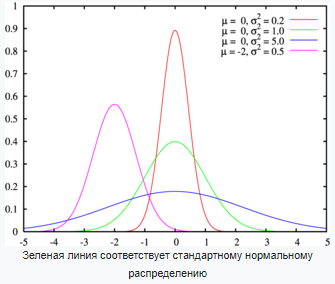
\includegraphics[width=10cm]{normal.png}
    \end{center}

    \begin{definition*}
        Введём понятие \textbf{Гамма-функции}.
        \begin{equation*}
            \Gamma(z) = \lim_{n \to +\infty} \frac{\left(n - 1\right)! n^z}{z(z+1)(z+2)\cdots(z + n - 1)},\hspace{1em} z \in \CC \setminus \left\{0,\ -1,\ -2, \ldots\right\}
        \end{equation*}        
    \end{definition*}

    \paragraph{Распределение Стьюдента}
    Пусть $Y_0,\ Y_1,\ \ldots,\ Y_n$~--- независимые стандартные нормальные случайные величины, такие что $Y_i \sim \mathcal{N}(0, 1),\ i = 0,\ldots,n$.
    Тогда распределение случайной величины $t$, где
    \begin{equation*}
        t={\frac {Y_{0}}{\sqrt {{\frac {1}{n}}\sum \limits _{i=1}^{n}Y_{i}^{2}}}},
    \end{equation*}
    называется \textbf{распределением Стьюдента} с $n$ степенями свободы $t \sim t(n)$.

    Это распределение абсолютно непрерывно с плотностью:
    \begin{equation*}
        \varrho_{t}(y)={\frac {\Gamma \left({\frac {n+1}{2}}\right)}{{\sqrt {n\pi }}\,\Gamma \left({\frac {n}{2}}\right)}}\,\left(1+{\frac {y^{2}}{n}}\right)^{-{\frac {n+1}{2}}},
    \end{equation*}
    где $\Gamma$~--- гамма-функция. Таким образом:
    \begin{equation*}
        \frac{\Gamma(\frac{ n+1}{2})} {\sqrt{ n\pi}\,\Gamma(\frac{ n}{2})} =  \frac{( n -1)( n -3)\cdots 5 \cdot 3} {2\sqrt{ n}( n -2)( n -4)\cdots 4 \cdot 2\,}, \text{ для чётных $n$}
    \end{equation*}
    и соответственно 
    \begin{equation*}
        {\frac {\Gamma ({\frac {n+1}{2}})}{{\sqrt {n\pi }}\,\Gamma ({\frac {n}{2}})}}={\frac {(n-1)(n-3)\cdots 4\cdot 2}{\pi {\sqrt {n}}(n-2)(n-4)\cdots 5\cdot 3\,}}, \text{ для нечётных $n$.}
    \end{equation*}
    \begin{center}
        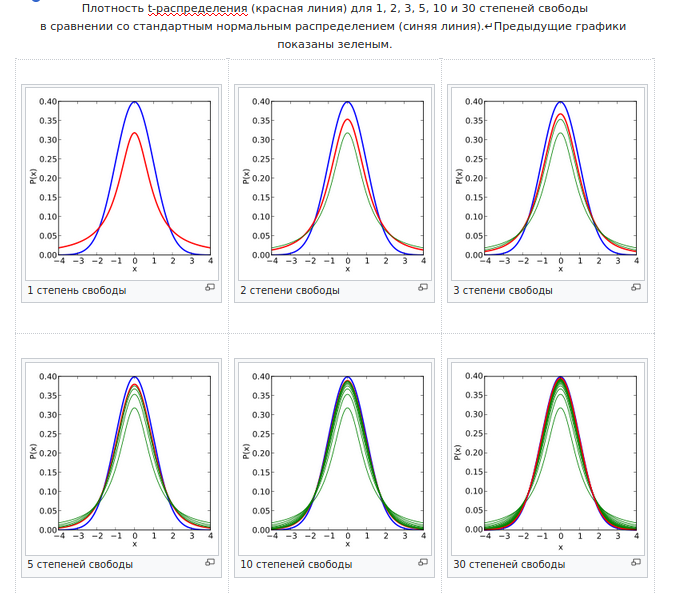
\includegraphics[width=15cm]{student.png}
    \end{center}

    \paragraph{Распределение хи-квадрат} Пусть $z_1, \ldots, z_k$~--- совместно независимые стандартные нормальный случайные величины, то есть $z_i \sim \Norm(0, 1)$. Тогда случайная величина 
    \begin{equation*}
        x = z_1^2 + \ldots + z_k^2
    \end{equation*}
    имеет \textbf{распределение хи-квадрат} c $k$ степенями свободы, то есть $x \sim \varrho_{\chi^2(k)}(x)$ или, если записать по-другому:
    \begin{equation*}
        x = \sum\limits_{i=1}^k z_i^2 \sim \chi^2(k)
    \end{equation*}

    Плотность распределения хи-квадрат имеет вид:
    \begin{equation*}
        \varrho_{\chi^2(k)}(x) = \frac{(1/2)^{k \over 2}}{\Gamma\!\left({k \over 2}\right)}\, x^{{k \over 2} - 1}\, e^{-\frac{x}{2}}
    \end{equation*}
    \begin{center}
        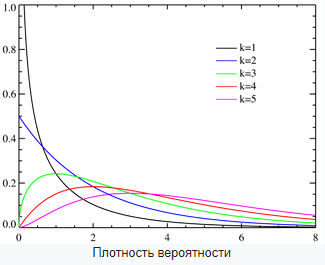
\includegraphics[width=10cm]{chi-square.png}
    \end{center}

    \begin{definition*}
        Введём понятие \textbf{Бета-функции}. 
        
        Формула через Гамма-функции:
        \begin{equation*}
            \Beta(x,y) = \frac{\Gamma(x) \Gamma(y)}{\Gamma(x + y)},
        \end{equation*}     
        где $\Gamma(x)$~--- Гамма-функция.
        
        Формула через нисходящий факториал:
        \begin{equation*}
            \Beta(x,y) = \frac{1}{y} \sum_{n=0}^{\infty} (-1)^n \frac{\left(y\right)_{n+1}}{n!\left(x + n\right)},
        \end{equation*}
        где $\left(x\right)_n$~--- нисходящий факториал, равный $x \cdot (x - 1) \cdot (x - 2) \cdot \ldots \cdot (x - n + 1)$.
    \end{definition*}
    
    \paragraph{Распределение Фишера}
    Пусть $Y_1,\ Y_2$~--- две независимые случайные величины, имеющие распределение хи-квадрат: $Y_i \sim \chi^2(d_i)$, где $d_i \in \NN,\ i = 1, 2$.
    Тогда распределение случайной величины 
    \begin{equation*}
        F = \frac{Y_1/d_1}{Y_2/d_2}
    \end{equation*}
    называется \textbf{распределением Фишера} со степенями свободы $d_1$ и $d_2$. Пишут $F \sim \Fshr(d_1, d_2)$.

    Опишем теперь функцию плотности случайной величины $F$:
    \begin{equation*}
        \varrho_F(x) = \frac{\sqrt{\frac{(d_1\,x)^{d_1}\,\,d_2^{d_2}}
        {(d_1\,x+d_2)^{d_1+d_2}}}}
        {x\,\mathrm{B}\!\left(\frac{d_1}{2},\frac{d_2}{2}\right)}
    \end{equation*}

    Картинка:
    \begin{center}
        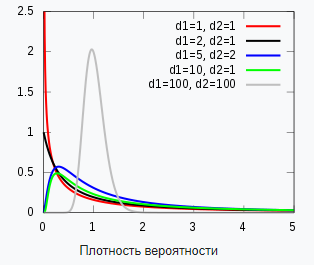
\includegraphics[width=10cm]{fisher.png}
    \end{center}

    \subsection{Совместное распределение случайных величин}
    Пусть $\xi$ и $\eta$~--- случайные величины. Рассмотрим отображение $\omega \to \left(\xi(\omega), \eta(\omega)\right)$. Это отображение определяет на плоскости вероятностную меру $\mu$ следующим образом:
    \begin{equation*}
        \mu(B) = \prob(\left\{\omega:\ \left(\xi(\omega), \eta(\omega)\right) \in B\right\})
    \end{equation*}
    Меру $\mu$ называют \textbf{совместным распределением} случайных величин $\xi$ и $\eta$. Функцию 
    \begin{equation*}
        F(x,y) = \mu(\left(-\infty, x\right] \times \left(-\infty, y\right]) = \prob(\left\{\omega:\ \xi(\omega) \leq x \text{ и } \eta(\omega) \leq y\right\})
    \end{equation*}
    называют \textbf{функцией совместного распределения} случайных величин $\xi$ и $\eta$.

    Аналогичным образом определяется совместное распределение любого конечного числа случайных величин.

    \subsection{Совместная и частная плотность}
    Если существует интегрируемая (по Риману) и неотрицательная функция $\varrho(x, y)$ такая, что 
    \begin{equation*}
        \mu(A) = \int \int_A \varrho(x, y) dx dy
    \end{equation*}
    для всякого допустимого (измеримого по Жордану) множества $A$, то $\varrho$ называется \textbf{совместной плотностью распределения}.

    Если известна плотность $\varrho$ совместного распределения $\xi$ и $\eta$, то можно найти плотности распределения каждой из случайных величин. Например, для случайной величины $\xi$:
    \begin{equation*}
        \mu_{\xi}(\left(a, b\right]) = \mu(\left(a, b\right] \times \RR) = \int_a^b \left(\int_{-\infty}^{+\infty} \varrho(x, y) dy\right) dx
    \end{equation*}
    и, следовательно,
    \begin{equation*}
        \varrho_\xi(x) = \int_{-\infty}^{+\infty} \varrho(x,y) dy
    \end{equation*}
    Если распределение каждой из случайных величин задаётся плотностью, то совместное распределение может не иметь плотность.

    \subsection{Независимые случайные величины и некореллированность случайных величин}
    Случайные величины $\xi$ и $\eta$ называются \textbf{независимыми}, если для всяких промежутков $U$ и $V$ выполняется равенство
    \begin{equation*}
        \prob(\left\{\omega:\ \xi(\omega) \in U \text{ и } \eta(\omega) \in V\right\}) = \prob(\left\{\omega:\ \xi(\omega) \in U\right\}) \cdot \prob(\left\{\omega:\ \eta(\omega) \in V\right\})
    \end{equation*}
    В терминах совместного распределения это равенство записывается так:
    \begin{equation*}
        \mu(U \times V = \mu_\xi(U) \cdot \mu_\eta(V)
    \end{equation*}
    Говорят, что мера $\mu$ является произведением мер $\mu_\xi$ и $\mu_\eta$ и пишут $\mu = \mu_\xi \otimes \mu_\eta$.

    Независимость $\xi$ и $\nu$ равносильна тому, что
    \begin{equation*}
        F(x, y) = F_\xi(x) \cdot F_\eta(y)
    \end{equation*}
    где $F$~--- совместная функция распределения $\xi$ и $\eta$.

    Для непрерывных случайных величин меняется определение математического ожидания. Математическое ожидание непрерывной случайной величины, распредление которой задаётся плотностью $\varrho(x)$, равно
    \begin{equation*}
        \mexp[\xi] = \int_{-\infty}^{+\infty} x \varrho(x) dx
    \end{equation*}
    Определения дисперсии, ковариации и коэффициента коррелляции требуют лишь дополнительного условия $\mexp \xi^2 < \infty$. Таким образом, определение некорреллированности случайных величин остаётся тем же: две случайные величины $X,Y$ называются \textbf{некорреллированными}, если $r(X, Y) = 0$. 

    Заметим, что если две случайные величины $X, Y$ независимы, то они некорреллированы. Обратное, вообще говоря, неверно.

    \subsection{Моменты распределений}
    Число $\mexp \xi^k$ называется \textbf{моментом порядка $k$} или \textbf{$k$-ым моментом случайной величины $\xi$}. 
\end{document}